\documentclass[oneside,12pt,fleqn]{memoir}
\usepackage{makeidx}
%\usepackage[utf8]{inputenc}
\pagestyle{plain}
%%%%%%%%%%%%%%%%%%%%%%%%%%%%%%%%%%% importa pacchetti
\usepackage{usepkg}
\usepackage{fancyfoot}
%%%%%%%%%%%%%%%%%%%%%%%%%%%%%%%%%%%%%
%%%%%%%%%%%%%%%%%% titletoc, titlesec setting
\usepackage{titleT}
%%%%%%%%%%%%%%%%%% setlength
\usepackage{mylength}
\linespread{0.5}
%%%%%%%%%%%% Hyperref package
\usepackage{hyperref}
\hypersetup{
    colorlinks,
    citecolor=black,
    filecolor=black,
    linkcolor=black,
    urlcolor=black
}
%%%%%%%%%%%%%%%%%%%%%%%%
%%%%%%%%%%%%%%%%%Geometry package
\usepackage{mygeometry}
%%%%%%%%%%%%%%%%%%%%%%%%%%%%%%%%%%% Funzioni per questo file main
\usepackage{LocalF}
%%%%%%%%%%%%%%%%%%%%%%%%%%%%%%%%%%% Funzioni generali
\usepackage{functions}
\usepackage{mathOp}
%http://tex.stackexchange.com/questions/246/when-should-i-use-input-vs-include
\usepackage{sources}
%%%%%%%%%%%%%%%%%%%%%%%%%%%%%%%%%

\makeindex
\raggedbottom %http://tex.stackexchange.com/questions/102084/annoying-paragraph-spacing-issue-with-memoir

\author{Pippetta}
\titleSounti per tesi eliosismologia}
\date{\today}

\begin{document}

\frontmatter


\maketitle


\tableofcontents*
\listoffigures

\mainmatter



\part{Cosa fare?

\subfile{intro}

\part{Tesina}

\subfile{helioSSMintro}


\chapter{Oscillazioni lineari adiabatiche. Modi di oscillazione.}
\PartialToc


\section{Per punti.}

\tool{
\begin{itemize}
    
    \item Perturbazioni: reazione del sistema: oscillazioni.
    
    \item Relazioni perturbazioni vs Langrangiana (Tolsoy): in entrambe introduco la perturbazione della posizione $\Lvar{\vec{\xi}}$, ma tolsoy gi\'a ignora la perturbazione di $g$.
    \item Adiabatic approximation: dalsgaard, stellar oscillation pg.47: why we can neglect heating term in energy equation.
    
    \item Nel caso di onde puramente acustiche
    \begin{align*}
    &\PtwoDy{t}{\rho'}=-v_S^2\nabla^2\rho'\intertext{equazione d'onda per la propagazione della perturbazione}\\
    &v_S=\sqrt{\frac{\Gamma_{1,0}P_0}{\rho_0}}&\intertext{adiabatic (Laplacian) sound speed.}
    \end{align*}

    Usando l'equazione di continuit\'a si vede che
    \begin{align*}
    &|\frac{\rho'}{\rho_0}|=\frac{v}{v_S}\\
    &|\frac{\rho'}{\rho_0}|\ll1\ \Rightarrow \ \frac{v}{v_S}\ll1
    \end{align*}
    La teoria lineare \'e valida finch\'e la velocit\'a delle fluttuazioni associata alle onde acustiche \'e minore rispetto alla velocit\'a del suono.
    Per l'equazione per la quantit\'a di moto linearizzata deve essere $\vec{c}\parallel \vec{k}$: la velocit\'a del fluido associato alle onde acustiche adiabatiche \'e parallela alla direzione di propagazione, sono ande di pressione.
    
    \item Forward problem: Matching accuracy of observations with accuracy of theoretical predictions.
    
    \item Metodo asintotico: varie approssimazioni. Accuratezza $10\%$. Le tecniche di inversione numerica hanno accuratezza \numrange{100}{1000} volte superiore ma dipende da un modello solare: dipendenza radiale dei coefficienti nelle equazioni delle oscillazioni.
    
    \item At observed solar frequencies the displacement at surface is approx. radial:
    
    \begin{equation*}
    \frac{\xi_h(R)}{\xi_r(R)}\approx\frac{GM}{R^3}\frac{L}{\omega^2}
    \end{equation*}
    
    \item L'approssimazione di Cowling \'e troppo grossolana se paragonata con l'accuratezza delle osservazioni \num{e-4}.
    (Vedi Robe68 JCD84)
    
    \item Confronto accuratezza asintotica vs numerica vs accuratezza osservazioni
    
    \item Procedure for determine n for computed modes of oscillation: Scufflaire 74, Osaki 75.
    
    \item Cowling approximation: System of equation of second order: Sturm-Liuville problem.
    \item Classification is invariant under continuus variation of equilibrium model: $\lambda=0$ Cowling approximation, $\lambda=1$ full case.
    
    \item Numerical inaccuracy: Van der raay, Palle roca cortes 1986.
    
    \item Mathematical classification often doesn't reflect the physical nature of the modes (Osaki75)
    
    \item Integrated energy: (relative) kinetic energy within a mode
    \begin{equation*}
    E_{n,l}=\frac{\int_0^R[\xi^2_r(r)+l(l+1)\xi_h^2(r)]\rho r^2\,dr}{4\pi M[\xi^2_r(R)+l(l+1)\xi_h^2(R)]}
    \end{equation*}
    
    \item dispersione energia del modo: effetti non adibatici (superficie), effetti non lineari (accoppiamento con altri modi, accoppiamento con flussi di materia)
    
    \item Trapping of modes.
    
    \item Reflection due to increase of $\omega_c$ in external layers before adiabatic approx break down: for what modes ??
    
    
    \item Identificazione dei modi: identificazione dei promontori nel diagramma \dgndi{} and of the lines in the power spectrum of the full disc oscillation signal.
    \item extrapolation to infinite number of grid points (shibahashi osaki 81)
    \item Pulsational unstable: self-excited oscillations.
    \item Eigenfrequencies for an infinite number of grid point is extrapolated $\nu_N=\nu_{\infty}+\frac{a}{N^2}$
    \item Forward problem: asymptotic expression for frequencies.
    \item dipendenza parametrica modello forward problem: asymptotic vs numerical.
\end{itemize}
}

In questa sezione descrivo le caratteristiche dei modi normali del Sole e come la struttura del interna del Sole influisce sulle frequenze.

Quando le frequenza sono molto grandi (per i modi p) o molto piccole (per i modi g) \'e possibile ricavare soluzioni analitiche approssimate delle equazioni delle oscillazioni. 

\section{Perturbazioni lineari adiabatiche.}

\subsection{Perturbatione dello stato di equilibrio.}

\begin{todo}{Cerca ampiezza media oscillazioni superficie ($\exv{v_{osc}}$)}
La piccola ampiezza delle oscillazioni giustifica l'uso solo del termine lineare dell'espansione.

\end{todo}

Descrivo le oscillazioni come piccole perturbazioni attorno allo stato di equilibrio stazionario (gli effetti non lineari sono dell'ordine di $\frac{v}{c_s}$ dove v \'e l'ampiezza dell'oscillazione):

\begin{align*}
&P(\vec{r},t)=P_0(\vec{r})+P'(\vec{r},t)&\intertext{$P'(\vec{r},t)$ \'e la perturbazione euleriana, quindi, detto $\delta\vec{\xi}$ lo spostamento della particella di fluido a causa della perturbazione}\\
&\Lvar{P(\vec{r})}=P(\vec{r}+\Lvar{\vec{\xi}})-P_0(\vec{r})=P'(\vec{r})+\Lvar{\vec{\xi}}\cdot\nabla P_0&\intertext{la velocit\'a dell'elemento di fluido dovuta alla perturbazione \'e}\\
&\vec{v}=\PDof{t}(\Lvar{\vec{\xi}})
\end{align*}

\begin{todo}{Particular solution/Perturbed solution}
Equations of conservation for stellar structure form a system of non-linear, partial differential equations. If an unperturbed solution is known we are often interested in finding another solution ''perturbed'' which differs only slightly from the unperturbed (we may think of the two solutions as representing possible future of the fluid differing from each others because of different initial conditions).

Expressing dependent variable of perturbed solutions as the sum of corr. dependent vars of unperturbed solution, neglecting all powers above the first and product of variations we obtain a system of partial differential equation whose solution gives the behaviour of the variation: the resulting set of equations is linear.

\end{todo}

Ricavo l'equazione del moto perturbato
\begin{align}
&\intertext{sostituisco nell'equazione del moto}
    &\rho\TDof{t}v\indices{_i}=\rho(\PDy{t}{v\indices{_i}}+v\indices{_j}\partial\indices{_j}v\indices{_i})=-\nabla P\indices{_i}+\rho\vec{g}\indices{_i}&\intertext{ le grandezze perturbate e sottraendo l'equazione statica ottengo}\nonumber\\
&\rho_0\PtwoDy{t}{\Lvar{\vec{\xi}}}=\rho_0\PDy{t}{\vec{v}}=-\nabla P'+\rho_0\vec{g}'+\rho'\vec{g}_0\label{eq:emper}\\
&\vec{g}'=-\nabla\Phi',\ \nabla^2\Phi'=4\pi G\rho'\nonumber
\end{align}

Analogamente per l'equazione di continuit\'a ottengo
\begin{equation}
\rho'+\div{(\rho_0\Lvar{\vec{\xi}})}=0\label{eq:contper}
\end{equation}

\subsection{Adiabatic approximation}

I tempi caratteristici per scambio di calore sono maggiori del periodo delle pulsazioni


\begin{align*}
&\TDy{t}{q}=\frac{1}{\rho(\Gamma_3-1)}(\TDy{t}{P}-\frac{\Gamma_1P}{\rho}\TDy{t}{\rho})=\epsilon-\frac{1}{\rho}\scap{\nabla}{F}&\intu{energy equation (rate heat gain/loss)}\\
&\frac{1}{\rho c_P}\nabla\cdot(\frac{4acT^3}{3\kappa\rho}\nabla T)\approx\frac{4acT^4}{3\kappa\rho^2c_PH}=\frac{T}{\tau_R}&\intertext{$\tau_R$ tempo scala radiativo, H lunghezza caratteristica, in cgs:}\\
&\tau_R=\num{e12}\frac{\kappa\rho^2H^2}{T^3}
\end{align*}

Per valori caratteristici solari ($\kappa=1$, $\rho=1$, $T=\num{e6}$, $H=\num{e10}$) ho $\tau_R\approx\SI{e7}{\year}\approx\tkh{}$, per valori caratteristici della zona convettiva ($\kappa=100$, $\rho=\num{e-5}$, $T=\num{e4}$, $H=\num{e9}$) ho $\tau_R\approx\SI{e3}{\year}\approx\tkh{}$.


In the inner part the nuclear term correspond to characteristic time $\tau_{\epsilon}\approx\frac{c_PT}{\epsilon}\approx\tkh{}$.

Confronto $\frac{T}{\tau_R}$, $\frac{T}{\tau_{\epsilon}}$ con $\TDy{t}{T}\approx\frac{T}{\Pi_{osc}}$ con $\Pi_{osc}\approx\si{\minute}-\si{\hour}$: heating term is generally very small compared with time derivative term.

Il moto di una elemento di fluido \'e descritto dalla relazione adiabatica


\begin{align*}
&\TDy{t}{P}=\frac{\Gamma_1P}{\rho}\TDy{t}{\rho}
\end{align*}

Approssimazione adiabatica non pi\'u valida vicino alla superficie solare dove i tempi per lo scambio di calore sono pi\'u brevi.

La condizione di perturbazione adiabatico linearizzata \'e
\begin{align}
&\PDy{t}{\Lvar{P}}-\frac{\Gamma_{1,0}P_0}{\rho_0}\PDy{t}{\Lvar{\rho}}=0\nonumber&\intertext{che integrata rispetto a t ed in funzione della variazione euleriana diventa}\nonumber\\
&P'+\Lvar{\vec{\xi}}\cdot\nabla P_0=\frac{\Gamma_{1,0}P_0}{\rho}(\rho'+\Lvar{\vec{\xi}}\cdot\nabla\rho_0)\label{eq:adper}
\end{align}

\subsection{Separazione variabili spaziali e temporali.}

Dall'equazione del moto \ref{eq:emper} si vede che
\begin{align*}
&\hat{r}\cdot(\rot{\PtwoDy{t}{\vec{\xi}}})=0&\intertext{cio\'e}\\
&\PDof{\theta}(\sin{\theta}\xi_{\phi})-\PDy{\phi}{\xi_{\theta}}=0&\intertext{quindi \'e possibile ricavare la componente tangenziale della perturbazione da una funzione scalare e dato che sono interessato alle oscillazioni }\\
&\vec{\xi}=\exp{i\omega t}(\xi_r(r),\xi_h(r)\PDof{\theta},\frac{\xi_h(r)}{\sin{\theta}}\PDof{\phi})Y_l^m(\theta,\phi)&\intertext{Ho introdotto le funzioni armoniche sferiche che soddisfano:}\\
&L^2Y_l^m=-\frac{1}{\sin{\theta}}\PDof{\theta}(\sin{\theta}\PDy{\theta}{Y_l^m})\\
&+\frac{1}{\sin^2{\theta}}\PtwoDy{\phi}{Y_l^m}=-r^2\nabla_h^2Y_l^m=l(l+1)Y_l^m
\end{align*}

La variazione euleriana di densit\'a, pressione, potenziale gravitazionale sono espressi
\begin{align*}
&(\rho_1,P_1,\Phi_1)=\exp{i\omega t}[\rho_1(r),P_1(r),\Phi_1(r)]Y_l^m
\end{align*}

\subsection{Frequenze di oscillazione discrete.}

Utilizzo l'equzione del moto ~\ref{eq:emper} e l'equazione di continui\'a~\ref{eq:contper} per eliminare $\xi_h(r)$ dall'equazione del moto
\begin{align}
&\frac{1}{r^2}\TDof{r}(r^2\xi_r)-\frac{\xi_rg}{c^2}+\frac{1}{\rho_0}(\frac{1}{c^2}-\frac{l(l+1)}{r^2\omega^2})P_1\nonumber\\
&-\frac{l(l+1)}{r^2\omega^2}\Phi_1=0\nonumber\\
&\frac{1}{\rho_0}(\TDof{r}+\frac{g}{c^2})P_1-(\omega^2-N^2)\xi_r+\TDy{r}{\Phi_1}=0\label{eq:eigenomega}\\
&\frac{1}{r^2}\TDof{r}(r^2\TDy{r}{\Phi_1})-\frac{l(l+1)}{r^2}\Phi_1-\frac{4\pi G\rho_0}{g}N^2\xi_r\nonumber\\
&-\frac{4\pi G}{c^2}P_1=0\nonumber
\end{align}

ho definito $N^2=g(\frac{1}{\Gamma_1P_0}\TDy{r}{P_0}-\frac{1}{\rho_0}\TDy{r}{\rho_0})$ e $S_l^2=\frac{l(l+1)c^2}{r^2}\approx k_h^2c^2$ con

\begin{align*}
&g=-\frac{1}{\rho_0}\TDy{r}{P_0}\\
&c^2=\frac{\Gamma_1P_0}{\rho_0}
\end{align*}


Il sistema di equazione ~\ref{eq:eigenomega} ha soluzione con le opportune equazioni al contorno per un insieme discreto di valori delle frequenze $\omega_{nlm}$, l'ordine angolare non compare nelle equazioni quindi gli autovalori $\omega_{nlm}$ sono $2l+1$ degeneri.

\subsection{Condizioni al contorno}

Abbiamo bisogno di 4 condizioni

\begin{itemize}
\item Due condizioni per $r=0$ punto regolare: le perturbazioni sono non singolari al centro del Sole, $r=0$.

\begin{equation*}
P'=0,\ \Phi'=0
\end{equation*}

Expansion near zero of solutions

\begin{align*}
&(l\neq0):\ \xi_r\propto r\expy{l-1};\ (l=0):\ \xi_r\propto r\\
&P',\ \Phi'\propto r^l
\end{align*}

\item Alla superficie solare richiediamo la continuit\'a di $\Lvar{\nabla\Phi}$ e che non si abbia dispersione verso l'esterno.

Outside the star $\rho'=0$ and Poisson equation can be solved by solution vanishing at infinity $\Phi'=Ar\expy{-l-1}$:
\begin{equation*}
\TDy{r}{\Phi'}+\frac{l+1}{r}\Phi'=0,\ r=\rsun{}    
\end{equation*}

The second condition depends on treatment of stellar atmosphere (Vedi chap 5 of lecture note on stellar oscillations: pg 103, (5.50)). It's reasonable that the boundary is free, no force acts on it: the star can be considered an isolated system. This is equivalent to requiring pressure constant at perturbed surface.

\begin{align*}
&\Lvar{P}=P'+\xi_r\TDy{r}{P}=0
\end{align*}

\end{itemize}

\subsection{Variabili adimensionali.}

Introduco le variabili adimensionali, che caratterizzano la perturbazione

\begin{align*}
&\eta_1=\frac{1}{r}\xi_r\\
&\eta_2=\frac{1}{gr}(\frac{P'}{\rho}+\Phi')\\
&\eta_3=\frac{1}{gr}\Phi'\\
&\eta_4=\frac{1}{g}\PDy{r}{\Phi'}\\
&\eta_i=\eta_i(r)Y_l^m(\theta,\phi)\exp{i\omega t}
\end{align*}

e riscrivo l'equazione del moto

\begin{equation*}
-\frac{\omega^2}{g}\vec{\xi}=[W(\eta_1-\eta_2+\eta_3)+(1-U)\eta_2]\hat{r}-r\nabla\eta_2
\end{equation*}

in funzione delle grandezze $U,V,W$ che caratterizzano lo stato di equilibrio del Sole

\begin{align*}
&U=\frac{r}{m}\PDy{r}{m}=\frac{1}{g}\PDy{r}{(gr)}\\
&V=-\frac{r}{P}\PDy{r}{P}=\frac{g\rho r}{P}\\
&W=\frac{r}{\rho}\PDy{r}{\rho}-\frac{r}{P\gamma_{Ad}}\PDy{r}{P}
\end{align*}

posto $\gamma_{ad}=\Dcvar{\TDly{\rho}{P}}{ad}=\Gamma_1$

La parte tangenziale dell'equazione del moto
\begin{align*}
&\frac{\omega^2}{g}\xi_{\theta}=\PDy{\theta}{\eta_2},\ &\frac{\omega^2}{g}\xi_{\phi}=\frac{1}{\sin{\theta}}\PDy{\phi}{\eta_2}
\end{align*}
sostituita nell'equazione di continuit\'a ($\scap{\nabla}{\xi}$), definita la frequenza adimensionale 
\begin{equation*}
\frac{\omega^2r}{g}=C\sigma^2:\ \sigma^2=\omega^2\frac{R^3}{GM}
\end{equation*}

permette di eliminare la dipendenza dalle variabili angolari
\begin{align*}
&r\PDy{r}{\eta_1(r)}=(3-\frac{V}{\gamma_{Ad}})\eta_1(r)+[\frac{l(l+1)}{C\sigma^2}\\
&+\frac{V}{\gamma_{Ad}}]\eta_2(r)-\frac{V}{\gamma_{Ad}}\eta_3
\end{align*}

mentre la parte radiale dell'equazione del moto

\begin{equation*}
r\PDy{r}{\eta_2(r)}=(W+C\sigma^2)\eta_1(r)+(1-U-W)\eta_2(r)+W\eta_3
\end{equation*}

dalla definizione di $\eta_3$

\begin{equation*}
r\PDy{r}{\eta_3}=(1-U)\eta_3(r)+\eta_4
\end{equation*}

infine l'equazione di Poisson \'e equivalente a
\begin{equation*}
r\PDy{r}{\eta_4}=-UW\eta_1+\frac{UV}{\gamma_{Ad}}\eta_2+[l(l+1)-\frac{UV}{\gamma_{Ad}}]\eta_3-U\eta_4
\end{equation*}



Abbiamo ottenuto quattro equazioni differenziali a coefficienti reali che dipendono dallo stato di equilibrio del modello stellare per le variabili adimensionali $\eta_i(r)$: un problema agli autovalori per $\sigma^2$, si pu\'o vedere che \'e autoaggiunto e quindi le autofunzioni corrispondenti ad autovalori diversi sono ortogonali: gli autovalori sono reali quindi posso avere un comportamento oscillante nel caso di stabilit\'a o esponenziale nel caso instabile.

Il sistema non dipende da m: le soluzioni sono $(2l+1)$ volte degeneri: la degenerazione \'e rimossa dalla rotazione ($\frac{\Omega}{\omega}\approx\num{e-4}$) o effetti gravitazionali di altri corpi.


\section{Stabilit\'a dei modi di oscillazione.}

\begin{todo}{Stabilit\'a oscillazioni nonradiali adiabatiche}

\end{todo}

\section{Propriet\'a generali delle oscillazioni adiabatiche.}

\begin{todo}{Frequenza di \bv{}.}
qui o nella sottosezione precedente??
Kippenhan: 40.3, eigenspectra
Dalsgaard: notes 5.3Pg 83-
\end{todo}

\begin{figure}[!ht]
\centering
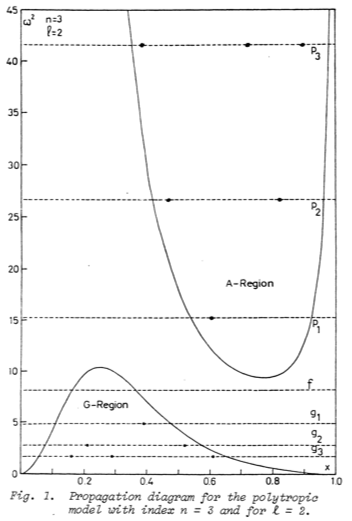
\includegraphics[width=\textwidth, height=0.9\textheight,keepaspectratio]{propagationAG}
\caption{Regioni di propagazione.}
\end{figure}


\begin{todo}{dalsgaard 2005}
homology argument: scaling factor $\sqrt{GM}$
\end{todo}


\begin{todo}{Soluzioni numeriche e comportamentpo asintotico}
La soluzione numerica \'e dipendente dal modello di equilibrio: per il modello stellare $M4K$ viene riportata un precisione di $\SI{0.02}{\micro\hertz}$ (accuratezza \num{e-5}), mentre differenti valori della costante G fra quelli usati in letteratura risultano in differenze nelle frequenze calcolate di \numrange{-0.35}{-0.08}\si{\micro\hertz}, maggiori di quelle che risultano da differenti schemi di integrazione numerica.
\end{todo}

\begin{todo}{Numerical technique}
Inter-comparison of the g-, f- and p-modes calculated using different oscillation codes for a given stellar model

\end{todo}

\begin{todo}{Continous variation of parameter}
Problems in cowling vs full
\end{todo}

La soluzione numerica delle equazioni \eqref{eq:eigenomega}



\begin{figure}[!ht]
\centering
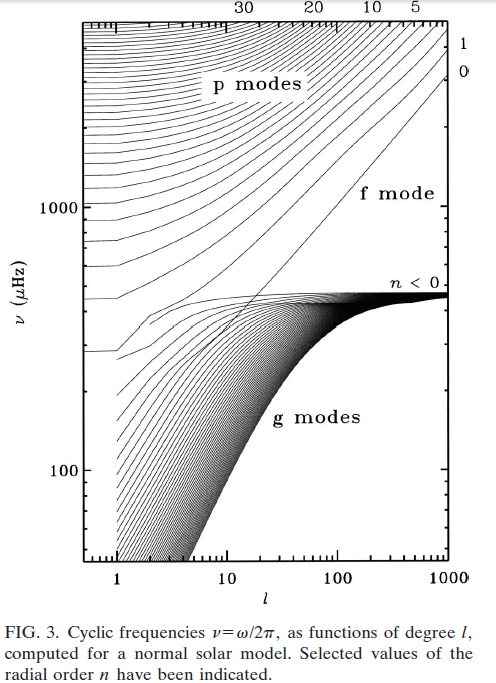
\includegraphics[width=\textwidth, height=0.9\textheight,keepaspectratio]{omega-l}
\caption{Modi di oscillazion. plot omega vs l..}
\end{figure}

mostra due differenti comportamenti. Uso l'approssimazione asintotica per determinare la natura delle oscillazioni nelle due zone.

\clearpage

\subsection{Comportamento asintotico}


Per determinare la struttura dello spettro delle oscillazioni introduciamo l'approssimazione di Cowling (\cite{cow41oscillations}) cio\'e trascuriamo la perturbazione del potenziale gravitazionale. Quindi il sistema si riduce al secondo ordine

\begin{align}
&\frac{1}{r^2}\TDof{r}(r^2\xi_r)-\frac{\xi_rg}{c^2}+\frac{1}{\rho_0}(\frac{1}{c^2}-\frac{l(l+1)}{r^2\omega^2})P_1=0\label{eq:cowosc}\\
&\frac{1}{\rho_0}(\TDof{r}+\frac{g}{c^2})P_1-(\omega^2-N^2)\xi_r=0\nonumber
\end{align}

Considero i limiti asintotici di alte e basse frequenze: in entrambi ottengo un problema del tipo di Sturm-Liuville

\begin{todo}{Sturm-Liouville theory}
%https://en.wikipedia.org/wiki/Sturm%E2%80%93Liouville_theory
\end{todo}

\begin{todo}{Modi stabili/instabili}
Cox ??
\end{todo}

\begin{itemize}
\item Per $\omega\to\infty$:

Lo spettro \'e discreto con punto di accumulazione a $\omega=\infty$.
Le oscillazioni sono prodotte da onde acustiche in cui la forza dominante \'e fornita dalla pressione, chiamati modi p, ordinati in base al numero di zeri di $\xi_r$ fra il centro e la superficie. I modi p sono stabili.

\item Per $\omega\to0$:

Lo spettro \'e discreto con punto di accumulazione a $\omega=0$.
Il moto \'e determinato dalla forza di gravit\'a, chiamati modi g (ordinati secondo il numero di nodi radiali). La stabilit\'a dei modi g \'e detrminata dalla stabilit\'a convettiva: dato che $\omega^2_{Ad}=-grW$ il criterio di instabilit\'a convettiva si traduce in $rW>0$. Se $W<0$ in tutta la stella tutti i modi g sono stabili ($g_+$), se esistono zone in cui $W>0$ esistono anche modi g instabili ($g_-$).
\end{itemize}

Lo spettro solare \'e la combinazione dei modi parziali precedenti; il modo f separa  i modi g e p: non ha nodi in direzione radiale.

\subsection{Relazione di dispersione per i modi gravo-acustici.}

Approssimo il comportamento spaziale delle oscillazioni con quello di onda piana
\begin{align*}
&\vec{\xi}\propto\exp{i\scap{k}{x}},\ \vec{k}=k_r\hat{r}+\vec{k}_h\\
&S_l^2=\frac{l(l+1)c^2}{r^2}\approx k_h^2c^2
\end{align*}
e i coefficienti delle equazioni \ref{eq:cowosc} costanti ( approssimazione valida se la lunghezza d'onda delle perturbazioni \'e molto minore della scala caratteristica di variazione dei coefficienti).

\begin{todo}{Per poter parlare di onde}
Per poter parlare di onde devo assumere che la variazione di $P_0$ e $\rho_0$ abbiano lunghezze caratteristiche maggiori delle lunghezze di interesse (short-wave acustic):
\begin{align*}
&\PtwoDy{t}{\rho'}=-v_S^2\nabla^2\rho'\intertext{equazione d'onda per la propagazione della perturbazione}\\
&v_S=\sqrt{\frac{\Gamma_{1,0}P_0}{\rho_0}}&\intertext{adiabatic (Laplacian) sound speed.}
\end{align*}



Usando l'equazione di continuit\'a si vede che
\begin{align*}
&|\frac{\rho'}{\rho_0}|=\frac{v}{v_S}\\
&|\frac{\rho'}{\rho_0}|\ll1\ \Rightarrow \ \frac{v}{v_S}\ll1
\end{align*}
La teoria lineare \'e valida finch\'e la velocit\'a delle fluttuazioni associata alle onde acustiche \'e minore rispetto alla velocit\'a del suono.
Per l'equazione per la quantit\'a di moto linearizzata deve essere $\vec{c}\parallel \vec{k}$: la velocit\'a del fluido associato alle onde acustiche adiabatiche \'e parallela alla direzione di propagazione, pressure force supply the restoring force.

\end{todo}

Manipolando il sistema \ref{eq:cowosc} inserendo perturbazioni della forma (conservazione energia) $\xi_r\propto\rho_0\expy{-\frac{1}{2}}\exp{ik_rr}$, $P_1\propto\rho_0\expy{\frac{1}{2}}\exp{ik_rr}$:

\begin{align*}
&\frac{1}{r^2}\TDof{r}(r^2\xi_r)-\frac{\xi_rg}{c^2}+\frac{1}{\rho_0}(\frac{1}{c^2}-\frac{l(l+1)}{r^2\omega^2})P_1=0\\
&\frac{1}{\rho_0}(\TDof{r}+\frac{g}{c^2})P_1-(\omega^2-N^2)\xi_r=0\\
\\
&\xi_r=\frac{1}{(\omega^2-N^2)}[\frac{1}{\rho_0}(\TDof{r}+\frac{g}{c^2})]P_1\\
&\TDof{r}\xi_r=-\frac{2}{r}\xi_r+\frac{\xi_rg}{c^2}+\frac{1}{\rho_0}(\frac{1}{c^2}+\frac{l(l+1)}{r^2\omega^2})P_1\\
\\
&\TDof{r} \frac{1}{\rho_0}(\TDof{r}+\TDof{r} \frac{g}{c^2})P_1-(\omega^2-N^2)\TDof{r} \xi_r=0
\end{align*}

\begin{todo}{relazione dispersione stix pg 156 (5.33)}

Gough pg 792 eq 25-26

\end{todo}

Se considero $g$, $N$ e $c$ lentamente variabili rispetto alla lunghezza d'onda delle perturbazioni lo stesso vale per la lunghezza caratteristica della densit\'a $H=-\frac{\rho_0}{\TDy{r}{\rho_0}}=(\frac{g}{c^2}+\frac{N^2}{g})\expy{-1}$ e la frequenza di taglio acustica $\omega_A=\frac{c}{2H}$. Scrivo la relazione di dispersione

\begin{align}
&k_r^2=\frac{\omega^2-\omega_A^2}{c^2}+S_l\frac{N^2-\omega^2}{c^2\omega^2}\label{eq:localdispersion}\\
&=\frac{\omega^2}{c^2}(1-\frac{\omega_{l,+}^2}{\omega^2})(1-\frac{\omega_{l,-}^2}{\omega^2})\nonumber
\end{align}

\begin{figure}[!ht]
\centering
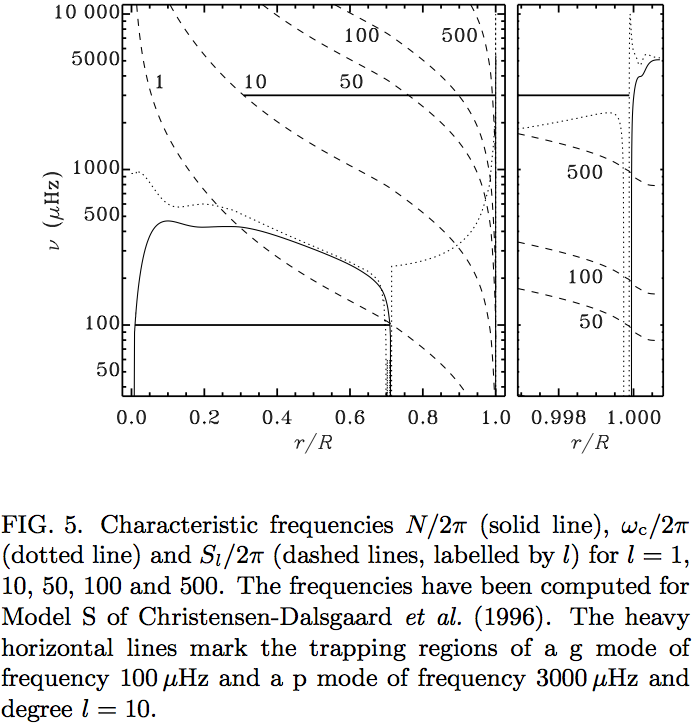
\includegraphics[width=\textwidth, height=0.9\textheight,keepaspectratio]{freqcaratt}
\caption{Frequenze caratteristiche.}
\label{fig:freqcaratt}
\end{figure}

\clearpage


\section{Regioni di propagazione.}

\begin{figure}[!ht]
\centering
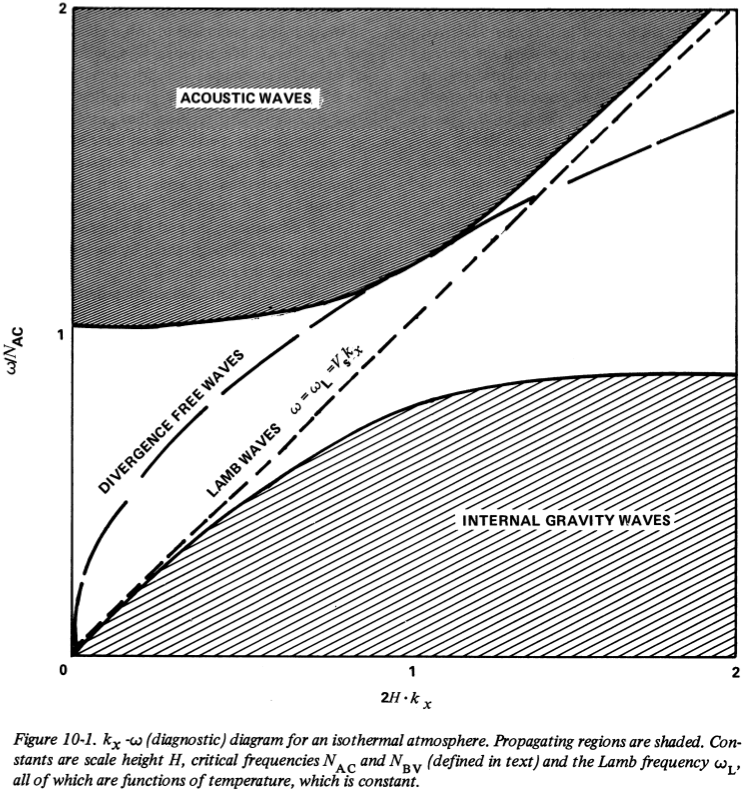
\includegraphics[width=\textwidth, height=0.8\textheight,keepaspectratio]{khomeagisot}
\caption{Diagramma frequenza numero d'onda orizzontale per atmosfera isoterma.}
\label{fig:khomeagisot}
\end{figure}

\begin{figure}[!ht]
\centering
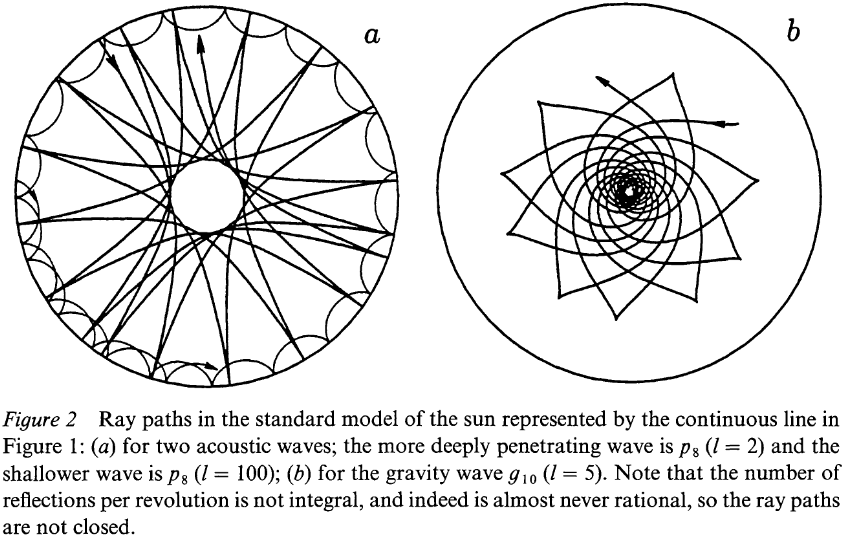
\includegraphics[width=0.9\textwidth, height=\textheight,keepaspectratio]{pgmodesC}
\caption{Cavit\'a risonanti per modi p e g.}
\label{fig:propagationAG}
\end{figure}

Il comportamento oscillatorio richiede $k_r^2>0$.

I punti di inversione per le onde acustiche sono definiti da 
\begin{align*}
    &\omega^2=\frac{l(l+1)c}{r^2}&\intertext{large $k_hH$}\\
    &\omega=\omega_A&\intertext{small $k_hH$}
\end{align*}

per i modi g da
\begin{align*}
    &\omega=N&\intertext{large $k_hH$.}
    &\omega=(\frac{\omega_A}{N})ck_h&\intertext{small $K_hH$.}
\end{align*}

\'E possibile analizzare tramite metodo  JWKB il sistema di equazioni delle oscillazioni del secondo ordine in approssimazione di Cowling, previa oppurtuna trasformazione, da cui si ottiene la relazione valida per i modi
\begin{equation}\label{eq:jwkb}
\omega\int_{r_1}^{r_2}[1-\frac{\omega_A^2}{\omega^2}-\frac{S_l^2}{\omega^2}(1-\frac{N^2}{\omega^2})]\expy{\frac{1}{2}}\frac{dr}{c}\approx\pi(n-\frac{1}{2})
\end{equation}
dove $r_1$ e $r_2$ sono due zeri consecutivi del numero d'onda radiale e l'integrazione \'e in una regione di propagazione. Nel caso dei modi p e assumendo $S_l\ll\omega$ vicino al punto di inversione superiore ho

\begin{equation}\label{eq:jwkbmodep}
\omega\int_{r_1}^{r_2}[1-\frac{S_l^2}{\omega^2}]\expy{\frac{1}{2}}\frac{dr}{c}\approx\pi(n-\alpha{\omega})
\end{equation}

\clearpage

\subsection{Cavit\'a acustiche.}
Per grandi $\omega$ ~\ref{eq:localdispersion} si riduce alla relazione di dispersione acustica 

\begin{equation*}
\omega^2=c^2(k_r^2+k_h^2)
\end{equation*}


Posso ricavare il raggio di inversione del moto in direzione radiale $k_r=0$ dalla relazione di dispersione per onde onde acustiche, da cui segue
\begin{equation}
\frac{c(r_i)}{r_i}=\frac{\omega}{l(l+1)}
\end{equation}

Maggiore \'e il grado l (piccolo $\lambda_h$) meno profonda \'e la cavit\'a: sono riflesse verso la superfice quando la velocit\'a del suono \'e aumentata fino alla loro velocit\'a di fase orizzontale; la profondit\'a della cavit\'a acustica varia con il variare della scala orizzontale dell'onda. (Top  convection zone down to the level at which refraction due to sound speed increasing $c\propto\sqrt{T}$ turn the wave around when $c=\frac{\omega}{k_h}$)

Stima profondit\'a cavit\'a acustica
\begin{align*}
    &T=\Dcvar{\TDy{z}{T}}{Ad}\delta&\intu{$\delta$ \'e la profondit\'a sotto la fotosfera}\\
    &T=\Dcvar{\TDy{z}{T}}{Ad}=\frac{T}{P}\TDly{P}{T}|_{Ad}\TDy{z}{P}=\frac{\gamma-1}{\gamma R}g=\frac{g}{c_P}\\
    &c^2=(\gamma-1)g\delta&\intertext{da $c=\frac{\omega}{k_h}$ segue:}\\
    &\delta=\frac{\omega^2}{k_h^2(\gamma-1)g}
\end{align*}
minore la lunghezza d'onda orizzontale pi\'u sottile la cavit\'a.

Vicino alla superficie l'efficienza della convezione diminuisce, il gradiente di temperatura diventa fortemente sopra-adiabatico e la fraquenza critica $\omega_A$ aumenta notevolmente: le onde acustiche con periodo attorno ai 5-min diventano evanescenti in poche scale di altezza: l'inizio della zona convettiva \'e uno specchio a larga banda per onde acustiche. 

Duvall82

In un grafico $\frac{\omega}{k_h}$ vs $\frac{\pi(n+\alpha)}{\omega}$ i modi p sono rappresentati da un'unica curva. Se considero la differenza di fase
\begin{align}\label{eq:duvall}
&\Delta\phi=\int_{r_t}^{\rsun{}}k_r\,dr=\int_{r_t}^{\rsun{}}(\frac{1}{c^2}-\frac{l(l+1)}{r^2\omega^2})\expy{\frac{1}{2}}\,dr\\
&=F(\frac{\omega}{L})\\
&\Delta\phi=\pi(n+\alpha)
\end{align}
tra i bordi interno ed esterno della cavit\'a acustica per un modo di oscillazione $\Delta\phi=\pi(n+\alpha)$ la costante $\alpha$ \'e necessaria dato che i bordi non sono rigidi.
L'integrale risulta funzione di $\frac{\omega}{k_h}$. 

\begin{figure}[!ht]
\centering
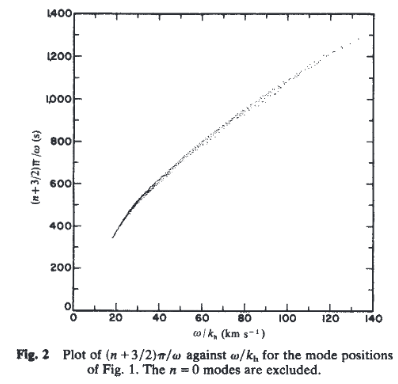
\includegraphics[width=\textwidth, height=0.9\textheight,keepaspectratio]{Duvall}
\caption{Legge di Duvall.}
\end{figure}

\clearpage

\subsection{Cavit\'a risonanti per modi g.}

Nella parte a basse frequenze dei modi g la relazione \ref{eq:localdispersion} si approssima, per $l\neq0$ con

\begin{equation*}
k_r^2=\frac{S_l^2}{c^2}(\frac{N^2}{\omega^2}-1)
\end{equation*}

La regione dei modi g ha come limite superiore N per grandi l, la linea $\omega=\frac{S_lN}{\omega_A}$.

Per i modi g le regioni di propagazione sono quelle per la frequenza \'e minore di entrambi $N$ e $ck_h$.

La struttura degli strati esterni del sole \'e dominata dalla ionizzazione di H e He con conseguente aumento dell'opacit\'a e quindi del gradiente di temperatura in equilibrio radiativo e il calore specifico: il gradiente di temperatura critico per instabilit\'a convettiva $\frac{g}{c_P}$ diminuisce. In questa regione il gradiente di temperatura \'e debolmente super-adiabatico, $N^2<0$: la zona convettiva costituisce una barriera per le onde di gravit\'a interne.

Le onde di gravit\'a sono presenti nelle regioni in cui il gas \'e neutro o completamente ionizzato ($N^2$ grande) e sono riflesse in regioni dove $N$ \'e piccolo o immaginario: ionizzazione parziale, instabilit\'a convettiva, centro del Sole.

Ho cavit\'a risonanti per modi g:
\begin{itemize}
    \item Core radiativo.
    
    Tra la la parte centrale dove $g\to0$ e il fondo della zona convettiva dove $N^2<0$.
    \item Atmosfera.
    
    $N$ ha un massimo in coincidenza del punto $T_m$ nella cromosfera: modi g confinati tra zona convettiva e cromosfera ($\Pi\approx\numrange{180}{800}\si{\second}$).
\end{itemize}


\section{Analisi asintotica}

\begin{todo}{Analisi asintotica}
Vedi stix 5.3??

Heliosismic inference: observed vs predicted frequencies (Simple models and analytic (asyntotic) formula).
\end{todo}

\subsection{JWKB analysis}

\begin{todo}{cos'\'e l'analisi asintotica}
Vedi articolo gough07
\end{todo}

Nell'analisi tramite JWKB si tiene conto del fatto che le oscillazioni non sono puramente acustiche e le propriet\'a del gas non sono omogenee.

I modi osservati sono di alto ordine radiale o grado angolare: uso l'approssimazione di Cowling (ignoro la perturbazione al potenziale gravitazionale $\Phi'$).

\begin{align*}
&\omega\int_{r_1}^{r_2}\sqrt{1-\frac{\omega_c^2}{\omega^2}-\frac{S_l^2}{\omega^2}(1-\frac{N^2}{\omega^2})}\,\frac{dr}{c}\approx\pi(n-\frac{1}{2})\\
&\omega_c=\frac{c^2}{4H^2}(1-2\TDy{r}{H})\\
&H=-(\TDy{r}{\ln{\rho}})\expy{-1}
\end{align*}

\subsection{Asymptotic properties of p modes}

Posso trascurare N e, eccetto vicino alla superficie, $\omega_c\ll\omega$, mentr vicino alla superficie $S_l\ll\omega$ for small/moderate l.

\begin{align*}
&\omega\int_{r_1}^{r_2}\sqrt{1-\frac{\omega_c^2}{\omega^2}-\frac{S_l^2}{\omega^2}}\,\frac{dr}{c}\approx\pi(n-\frac{1}{2})&\intertext{where $r_1=r_t$, $r_2=R_t$. With help of our assumption we can expand the integral and, introducing the function $\alpha(\omega)$ depending only on frequency and near surface behaviour of $\omega_c$.}
\end{align*}

For low degree modes we use the fact that integrand differs from 1 only close to lower turning point close to center for low order mode ($F(w)\approx\int_0^R\frac{dr}{c}-w\expy{-1}\frac{\pi}{2}$)

\begin{align*}
&\nu_{nl}=\frac{\omega_{nl}}{2\pi}\approx(n+\frac{l}{2}+\frac{1}{4}+\alpha)\Delta\nu\\
&\Delta\nu=[2\int_0^R\frac{dr}{c}]\expy{-1}&\intu{is the inverse of twice travel time center/surface. This equation predict uniform spacing in n of frequency of low degree modes (claverie79)}
\end{align*}

Deviazioni da questa legge hanno potenziale diagnostico per la parte interna, infatti estendendo l'espansione di

\begin{equation*}
F(w)=\int_{r_t}^R\sqrt{1-\frac{c^2}{w^2r^2}}\,\frac{dr}{c}
\end{equation*}

fino al termine dipendente dalla variazione di c:

\begin{align*}
d_{nl}=\nu_{nl}-\nu_{n-1,l+2}\approx-(4l+6)\frac{\Delta\nu}{4\pi^2\nu_{nl}}\int_0^R\TDy{r}{c}\,\frac{dr}{c}&\intertext{sound speed is reduced as $\mu$ increases with H to He conversion as star ages: as a result $d_{nl}$ is reduced providing measure of evolutionary state of stars}
\end{align*}

\subsection{Asymptotic g modes}

In inner domain an expansion in terms of $\frac{\omega^2}{S_l^2}$ is possible, while $\frac{\omega^2}{N^2}$ serves as small expansion parameter in outer domain containing the surface, additional domains have to be considered for zeros of $N^2$

For the Sun we have $N^2(r_v)=0$ where $r_v$ marks lower bound of convection zone, matching the respective expansion we have in first order
\begin{align*}
&T_{n,l}=\frac{2\pi^2(n+\frac{l}{2}-\frac{1}{4})}{\sqrt{l(l+1)}}(\int_0^{r_v}\frac{N}{r}\,dr)\expy{-1}=\frac{n+\frac{l}{2}-\frac{1}{4}}{\sqrt{l(l+1)}}T_0
\end{align*}

g modes have equidistant period spacing.


\section{Excitation and damping. Ampiezza delle autofunzioni meccanismi di eccitazione delle oscillazioni solari.}

\subsection{$\kappa$ mechanism}

Suppose in phase of comperession opacity increases: the compressed layer then absorbs energy out of radiative flux toward stellar surface and thus will be heated in excess than mere adiabatic heating.

The subsequent compression will be stronger than preciding one.

\cite{zhe63variable} demonstrated that this mechanism of overstability drives the pulsation of $\delta$ cephei and related variable stars where is particularly effective in layer of He second ionization.

The crucial parameter measuring the opacity variation is 
\begin{equation*}
\kappa_T=\Dcvar{\PDly{T}{\kappa}}{P}
\end{equation*}

It has a maximum in the layer of partial H ionization: in this layer there is a strong driving but we must include contributions from all layers in order to see if a particular mode is excited or damping.

We must abandon adiabatic assumption and use actual energy equation: 
\begin{equation*}
c_P\rho(\PDy{t}{T}-\nad{}\frac{T}{P}\TDy{t}{P})=-\nabla\cdot\vec{F}
\end{equation*}
from \cite{and75nonadiabatic}: the second term on the left describes adiabatic heating/cooling and $\vec{F}$ is the energy flux.

Il sistema di equazioni che descrive le oscillazioni non e pi\'u autoaggiunto e le frequenze sono complesse.

\'e difficile determinare se un modo sia instabile o meno perch\'e \'e necessario tenere conto dello smorzamento causato dalle perdite radiative nell'atmosfera otticamente sottile e dell'interazione con i moti convettivi non stazionari: difficile da stimare.

Since relative growth rate are small, with $Q=\frac{\Re{\omega}}{\Im{\omega}}\approx10^3$ or larger for solar p modes there is not much certainty about sign of $\Im{\omega}$.

\subsubsection{Argument against excitation of solar p modes by means of $\kappa$ mechanism}

The excited/damped oscillator is represented by
\begin{equation*}
\ddot{\xi}-2\beta\dot{\xi}+\omega^2\xi=0
\end{equation*}

The net effects of all excitation and dumping yield the coefficient $\beta$: if excitation wins over damping $\beta>0$, then there is unlimited growth of this mode (the equation above is homogeneous and linear). It's only be means of non-linear terms neglected above and in oscillation equations that the growth could be held.

Before non-linear terms take effect the amplitud should be sizable unlike small amplitudes observed on the Sun.

\subsection{Stochastic excitation by convection}

L'interazione con la convezione e causa di smorzamento: un blob di gas che si muove avanti e indietro nel suo moto convettivo produce attrito come gli atomi agitati da moto termico e collisioni.

D'altra parte il gas racchiuso tra due pareti riflettenti \'e continuamente colpito/perturbato da blob di gas convettivi: analogo di una campana suona in maniera casuale a una trumphet excited with random spectrum and random phase jump.

Formalmente si descrive l'oscillatore con
\begin{equation*}
\ddot{\xi}-2\beta\dot{\xi}+\omega^2\xi=f(t)
\end{equation*}
dove $f(t)$ \'e una forzante stocastica.

The spectrum and amplitudes of excited modes is determined by forcing function.

Observed frequencies are in the range \SIrange{2}{5}{\milli\hertz}: the upper bound comes about because up to $l\approx2000$ ($2Hk_h\approx1$) the atmospheric acustic cutoff is at about \SI{5}{\milli\hertz} almost indipendent of horizontal wavenumber; at larger frequencies there is no total reflection and no eigenoscillations with discrete spectrum. For lower bound at about \SI{2}{\milli\hertz}: for high l there are no p modes at smaller frequencies, we see the smallest radial order including fundamental; at low l the oscillations of low frequencies have upper reflection boundariy so deep below photosphere that at observable layers the amplitude is undetectable with present technique.


\subsection{Wave propagation in atmosphere}

There is no acustic cutoff for frequencies higher than atmospheric value of $\omega_A$: instead of discrete eigenvalue we expect a continuum of propagating acustic waves clearly seen for frequencies above $\approx\SI{5}{\milli\hertz}$. The phase difference between two levels in atmosphere separated by $\Delta r$ is $\Delta\phi=k_r\Delta r$ and icreases with frequencies because $k_r\approx\frac{\omega}{c_s}$ at this high freq.

There is some phase propagation for frequencies below \SI{5}{\milli\hertz} within spectral band where discrete modes exist: the closer the frequency is to atmospheric $\omega_A$ the less perfect is the reflection of eigenmodes.

Staiger's diagram also indicates presence of IGW in solar atmosphere. The signature is the negative phase difference at low frequencies: using dispersion relation for isothermal atmosphere
\begin{equation*}
\frac{k_h^2(\omega^2-N^2)}{\omega^2(\omega^2-\omega_A^2)}+\frac{k_r^2}{\omega^2-\omega_A^2}=\frac{1}{c^2}
\end{equation*}
which for constant $\omega$ is a quadratic surface in $\vec{k}$ space.

The vector of phase propagation $\vec{k}$ is the radius vector, the group velocity, gradient $\PDy{\vec{k}}{\omega}$ is perpendicular to surface $\omega^2$ const.

In the region of propagating acustic wave the surfaces are oblate ellipsoid of revolution with respect to $k_r$ axis because $\omega^2>\omega_A^2$ (and $\omega^2>N^2$): in this case the vertical components of phase velocity and group velocity have the same sign.

A wave having its excitation deep in the atmosphere will propagate its energy upward and if it's of acustic nature will also propagate phase upward.

By contrast the obove dispersion relation will represent one-shell hyperboloid of revolution for IGW where $\omega^2<N^2$ (and $\omega^2<\omega_A^2$): the r component of phase and group velocity have different sign. An IGW excited from below with upward propagating energy will exhibits downward propagating phase (Vedi steigert intorno a \SI{1}{\milli\hertz}).

(IGW possible only for $N^2>0$ are in stably stratified layers the natural substitutes of convection which depends on $N^2<0$)

\subsection{$\epsilon$ mechanism}

The $\epsilon$ mechanism consist in amplified energy production in the phase of maximum compression (diesel engine): the mechanism would operate in region of max He3 accumulation and lead to growing perturbation because of strong T sensitive of \mblock{^3He(^3He,2p)\alpha} reaction of PPI chain. The g modes, having peak amplitude in deep core would most likely be excited.

Instability of g modes producing finite amplitude perturbation would destroy $^3He$ peak: intermittent manner with timescale approx \SI{e8}{\year}.


\chapter{Problema inverso: correzione al modello dalle oscillazioni.}
\PartialToc

\section{Per punti.}

\begin{itemize}
    
    \item astratto forme di inversione: 3 tipi. Primary inversion: asymptotic technique. Secondary inversion: impose thermal equilibrium, energy transport, equation of state, $\kappa$, $\epsilon$. Tertiary inversion impose that the evolution of the Sun is in accordance with standard model. Inversione fornisce dettagli sulla ''microfisica''.
    
    \item By determining frequency of p,g modes we can probe variation of $c(r)$ and $N$.
    \item Principio variazionale
    \item Tesseral modes ($m\neq0$) yield information about Sun's internal rotation and magnetic field (justified ignoring effects of centrifugal and Lorentz force on radial structure)
    \item Variational principle, model dependent inverion methods. Non ''perfetta corrispondenza'' nel modello solare.
    
    \item Rotation: relation data vs $\Omega(r)$ is linear to high approximation
    \begin{equation*}
    \Delta_i=\int_0^RK_i(r)\Omega(r)\,dr+\epsilon_i
    \end{equation*}
    $\Delta_i$ sono le frequenze osservate e $\epsilon_i$ l'errore sulle frequenze osservate.
    
    \item Dzi90: pressure, density in neutrino production regions: knowledge of these thermodynamic function doesn't suffice tpo determine T.
    
    \item Inversion methods: JCD85; Brodsky, Vorontsov 88; JCD, Gough, Thompson 88;  Vorontsov 88; Kosovichev 88; Gough Kosovichev 88.
    
    \item In determinati casi \'e sufficiente confrontare le differenze di frequenza $\delta_{nl}=\nu_{n,l}-\nu_{n-1,l+2}$ piuttosto che le frequenze assolute.
    
    \item Asymptotic method is not valid in innermost part of the Sun: Shibahashi sekii 88 (shart wavelength asymptotic); shibahashi 89; JCD 89 
    
    \item In the structure case relation between structure and multiplet is highly nonlinear.
    \item Exactly calculated eigenfunction: linearization about SSM.
    \item Averaged  multiplet $\nu_{nl}$ carry info about sherical symmetric component of solar structure: testin solar model, info about properties of matter in solar interior.
    \item $\Gamma_1$, $\rho$, $c$ are constrained by freq. directly.
    \item If equation of state and heavy elements abundances are known $\Gamma_1$ can be expressed in terms of a thermodynamical variable and $Y$: $(\frac{P}{\rho},Y)$, $(\rho,Y)$.
    
    \item Gough84:  Inversion of $F(w)$: $c(t)$ without reference to the model.
    
    \item Simple form of asymptotic analysis
    \begin{align*}
    &\frac{\pi(n+\alpha)}{\omega}\approx F(\frac{\omega}{L})\\
    &F(w)=\int_{r_t}^R\sqrt{1-\frac{c^2}{w^2r^2}}\frac{dr}{c}
    \end{align*}
    sistematic error.
    \item differential asymptotic inversion:
    \begin{align*}
    &S_{nl}\frac{\delta\omega_{nl}}{\omega_{nl}}\approx H_1(\frac{\omega_{nl}}{L})+H_2(\omega_{nl})\\
    &S_{nl}=\int_{r_t}^R(1-\frac{L^2c^2}{r^2\omega_{nl}^2})\expy{-\frac{1}{2}}\frac{dr}{c}-\pi\TDy{\omega}{\alpha}\\
    &H_1(w)=\int_{r_t}^R(1-\frac{c^2}{r^2w^2})\expy{-\frac{1}{2}}\frac{\delta_rc}{c}\frac{dr}{c}\\
    &H_2(w)=\frac{\pi}{\omega}\delta\alpha(\omega)
    \end{align*}
    
    \begin{figure}[!ht]
    \centering
    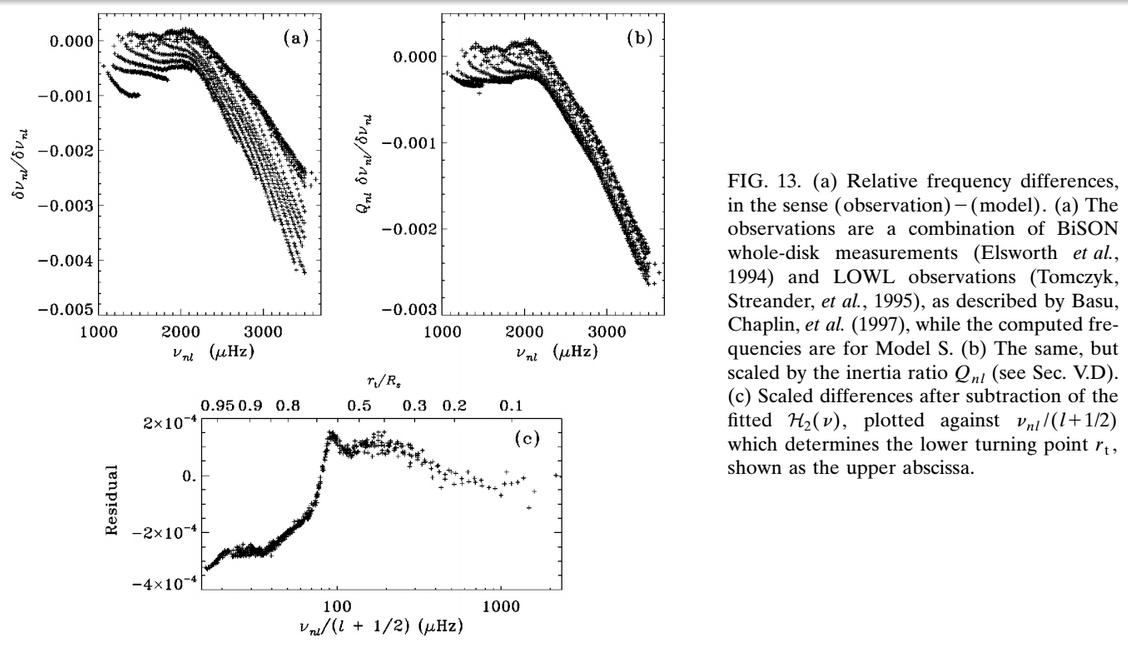
\includegraphics[width=\textwidth, height=0.9\textheight,keepaspectratio]{freqdiff_13}
    \caption{Frequency difference.}
    \end{figure}

    \clearpage
    
    Drastic change of behaviour for mode penetrating beneath base of convection zone
    
    \item $\nu$ sensitive to details of EOS (Berthomieu, lubow 80)
    \item Confronto densit\'a, velocit\'a del suono del modello vs quelle ottenute dalle frequenza misurate
    \item Frequency changes as linear functional of properties of the models (vedi stix 5.3 etc) for small changes.
    \item Changes to the properties of the model are directly infered from observations.
    \item tecniche di inversion. Classe coefficienti lineare: mola, sola, inversion of acustic data (Thomson 1993). Classe parametri lineare: regularized least square,statistical properties of inference from inversion.
    \item Result of inversion using SOLA fig 14
    \item Inversion technique to deduce interior structure and dynamics given frequencies and their splitting.
    \item Inside of our nearest star as gleaned from the study of its vibration.
    \item Fornisce strumente per scoprire dove il modello solare \'e deficitario (correzioni alla legge dei gas perfetti, Z, etc)
    \item chemical constitution low l p modes (Jimenez88, noel84).
    \item EOS: Electrostatic correct5ion to PG law (Debye-Huckel theory). Effects of electrostatic corrections upon eigenvalue spectrum of low degree p modes + Partial electron degeneracy.
    \item Gli aspetti della struttura solare sono determinati direttamente dai dati.
    \item Determinazione struttura idrostatica.
    \item Inversion of dynamical oscillation: relation between pressure and inertia density $\rho$.
    \item $\omega_{n,l}-\omega_{n-1,l+2}$: chemical inhomogeneities.
    \item Error to be assigned to helioseismological determination of physical quantities Q (characterizing solar structure).
    \item Errors evaluation: Var/CoVar matrix.
\end{itemize}


\section{Tecniche asintotiche.}

Per modi di basso grodo \'e possibile espandere al primo ordine l'integrale nella \ref{eq:duvall} $F(w)\approx\int_0^R\frac{dr}{c}-w\expy{-1}\frac{\pi}{2}$ ed esprimere la legge di Duvall tramite
\begin{equation}\label{eq:claverie}
    \nu_{nl}=\frac{\omega_{nl}}{2\pi}\approx(n+\frac{l}{2}+\frac{1}{4}+\alpha)\Delta\nu
\end{equation}
con $\Delta\nu=[\int_0^R\frac{dr}{c}]\expy{-1}$.
La presenza di picchi uniformemente spaziati di modi a basso grado l \'e stata osservata da Cleverie79.

Estendendo ancora l'espansione di \ref{eq:duvall} si ha una misura della variazione di $c$ nel core della stella
\begin{equation}\label{eq:tassoul}
    d_{nl}=\nu_{nl}-\nu_{n-1,l+2}\approx-(4l+6)\frac{\Delta\nu}{4\pi^2\nu_{nl}}\int_0^R\frac{dc}{dr}\frac{dr}{r}
\end{equation}
La velocit\'a del suono \'e ridotta a causa dell'aumentare di $\mu$ durante la fusione di H in He durante l'evoluzione stellare e quindi $d_{nl}$ \'e ridotto.

\begin{todo}{Analisi legge Duval }
Dalsnotes Pg 155
\end{todo}

\section{Linearizzazione della ''variazione'' attorno ad un modello solare.}

\subsection{Principio variazionale}

Riscrivo l'equazione del moto linearizzata nella forma
\begin{equation}
    \omega^2\Lvar{\vec{r}}=\frac{1}{\rho}\nabla p'-\vec{g}'-\frac{\rho'}{\rho}\vec{g}=\mathcal{F}(\Lvar{\vec{r}})
\end{equation}
da cui risulta che in seguito ad una perturbazione del modello di equilibrio $\Lvar{\mathcal{F}}$ le frequenze delle oscillazioni adiabatiche sono determinate da 

\begin{equation}\label{eq:variational}
    \Lvar{\omega^2}=\frac{\int_V\Lvar{\vec{r}}^*\cdot\mathcal{F}(\Lvar{\vec{r}})\rho\,dV}{\int_V|\Lvar{\vec{r}}|^2\rho\,dV}
\end{equation}
$\Lvar{\vec{r}}$ \'e autovalore per il problema imperturbato.




\section{Rotazione.}

Il Sole \'e un rotatore lento.



We want to find a velocity field which in spherical coordinates has the form
\begin{align*}
&\vec{v_0}=(0,0,r\Omega\sin{\theta})=\vecp{\Omega}{r}\\
&\vec{\Omega(r,\theta)}=(\Omega(r,\theta)\cos{\theta},-\Omega(r,\theta)\sin{\theta},0)&\intertext{il vettore velocit\'a angolare \'e funzione di r e $\theta$}
\end{align*}

Without rotation the inertia term is $\rho_0\TDy{t}{\vec{v}}=\rho_0\PtwoDy{t}{\vec{\xi}}$ where there is no mean motion, in case of rotation $\rho_0(\PDof{t}+\scap{v_0}{\nabla})^2\vec{\xi}$.

We consider additional term as a small perturbation

\begin{align*}
&\PDof{t}=i\omega\\
&\omega=\omega_{\alpha}+\Delta\omega_{\alpha}\\
&Y_{\alpha}=Y_{lm}\\
&\rho_0(\omega_{\alpha}^2+2\omega_{\alpha}\Delta\omega_{\alpha})\vec{\xi}\\
&=\nabla P_1-\frac{\rho_1}{\rho_0}\nabla P_0+\rho_0\nabla\Phi_1+2i\omega_{\alpha}\rho_0(\scap{v_0}{\nabla})\vec{\xi}&\intu{equazione del moto al primo ordine nella perturbazione}
\end{align*}

quindi risulta

\begin{align*}
&\Delta\omega_{\alpha}=\frac{i\int\rho_0\xi_{\alpha}^*(\scap{v_0}{\nabla})\xi_{\alpha}}{\int\rho_0\xi_{\alpha}^*\xi_{\alpha}}\\
&\Delta\omega_{\alpha}=\frac{-m\int\rho_0\Omega\xi_{\alpha}^*\xi_{\alpha}\,dV+i\int\rho_0\xi_{\alpha}^*(\vecp{\Omega}{\xi_{\alpha}})\,dV}{\int\rho_0\xi_{\alpha}^*\xi_{\alpha}}\intu{usando $\vec{v_0}=\vecp{\Omega}{r}$}
\end{align*}

Dobbiamo trovare $\Omega(r,\theta)$ dalla differenza $\Delta\omega_{\alpha}$: the problem is linear in $\Omega$ so the shift $\Delta\Omega_{\alpha}$ is of the same order as $\Omega$.

For evaluation of shift formula we must know eigenfunction $\xi_{\alpha}$ of unperturbed state.

Per rotazione puramente radiale $\Omega(r)$
\begin{align*}
&\Delta\omega_{\alpha}=-m\frac{\int_0^{\rsun{}}\rho_0\Omega\{|\xi_r-\xi_h|^2+[l(l+1)-2]|\xi_h|^2\}r^2\,dr}{\int_0^{\rsun{}}\rho_0\{|\xi_r|^2+l(l+1)|\xi_h|^2\}r^2\,dr}\\
&=\int_0^{\rsun{}}K_{\alpha}(r)\Omega(r)\,dr
\end{align*}

nel caso di rotazione dipendente solo da r $\Delta\omega_{\alpha}$ \'e lineare in m, $2l+1$ frequencies with equidistant spacing.

Any given $\Delta\Omega_{\alpha}$ samples angular velocity in the depth range corresponding to $\xi_{\alpha}$.

Le osservazioni della superficie mostrano una dipendenza dalla co-latitudine 

\begin{equation*}
\frac{\Omega(\theta)}{2\pi}=\SI{451.5}{\nano\hertz}-\SI{65.3}{\nano\hertz}\cos^2{\theta}-\SI{66.7}{\nano\hertz}\cos^4{\theta}
\end{equation*}

risultato di un best fit (discrepanze notevoli e variazioni temporali).

For an investigation of the full function $\Omega(r,\theta)$ the whole multiplet $2l+1$ frequencies must be used: deviation from equidistant spacing within the multiplet is typical of latitudinal shear.


\section{Inversione non asintotica.}

In the structure case the relation between structure and multiplet frequencies is highly nonlinear: we perform linearization on the assumption that a solar model close enough to actual solar structure exists.

\subsection{Correzioni struttra idrostatica}

\'E possibile quindi mettere in relazione la differenze tra le frequenze osservate  con quelle calcolate da un modello, $\delta\omega_{nl}=\Omega_{\odot}-\Omega_{Mod}$ e le differenze nella stratificazione idrostatica

\begin{align}
&\frac{\delta\omega_{nl}}{\omega_{nl}}=\int_0^R[K^{nl}_{c^2,\rho}(r)\frac{\delta_rc^2}{c^2}(r)+K^{nl}_{\rho,c^2}(r)\frac{\delta_r\rho}{\rho}(r)]\,dr\\
&+I_{nl}\expy{-1}F_{Surf}(\omega_{nl})\\
&\frac{\delta_rc^2}{c^2}(r)=\frac{[c_{\odot}^2(r)-c_{mod}^2(r)]}{c^2(r)}\\
&\frac{\delta_r\rho}{\rho}(r)=\frac{[\rho_{\odot}(r)-\rho_{mod}(r)]}{\rho(r)}\label{eq:invstructure}
\end{align}

i kernel $K_Q^j$ dipendono dalle autofunzioni del modello, il termine $I_{nl}\expy{-1}F_{Surf}(\omega_{nl})$, $I_{nl}=\int_V|\Lvar{\vec{r}}|^2\rho\,dV$ \'e una correzione dovuta alle differenti condizioni fisiche che si incontrano vicino alla superficie: per basse frequenze si ha riflessione pi\'u in profondit\'a a $\omega=\omega_c$ e quindi risentono meno degli effetti degli strati superficiali.

The analysis in terms of $\frac{\delta_rc^2}{c^2}(r)$ and $\frac{\delta_r\rho}{\rho}(r)$ capture the difference between Sun and model related hydrostatic structure.

\subsection{Correzioni equazione di stato e composizione.}

Since sound speed depends upon $\Gamma_1$ as $c_s^2=\Gamma_1\frac{P}{\rho}$ we can express $\Gamma_1(P,\rho,Y,Z)$ from thermodynamic properties and composition of the gas.

We obtain equivalent formulation of \ref{eq:invstructure} expressing $\delta_rc^2$ in terms of $\delta_rP$, $\delta_r\rho$, $\delta_rY$ and $\delta_r\Gamma_1$

\begin{align}
&\frac{\delta\omega_{nl}}{\omega_{nl}}=\int_0^RK^{nl}_{u,Y}(r)\frac{\delta_ru}{u}(r)\,dr+\int K^{nl}_{Y,u}(r)\delta_rY\,dr\\
&+\int_0^RK^{nl}_{c^2,\rho}(r)(\frac{\delta\Gamma_1}{\Gamma_1})_{int}\,dr+I_{nl}\expy{-1}F_{Surf}(\omega_{nl})\label{eq:diffthermo}&\intertext{allowance in error $(\delta\Gamma_1)_{int}$, difference between $\Gamma_1$ Sun and $\Gamma_1$ model EOS.}
\end{align}

Fatti:
\begin{itemize}
    \item Inversione di $\Gamma_1$ mostra la necessit\'a di tener conto degli effetti relativistici per gli elettroni (average thermal energy approx \SI{1.35}{\kilo\ev} approx $0.3\%$ of $m_e$).
\end{itemize}


\section{(Numerical) Inversion technique.}

\subsection{Least square inversion.}

Parametrize unknown functions $\frac{\delta_rc^2}{c^2}$, $\frac{\delta_r\rho}{\rho}$, $F_{Surf}$ (Slowly variable polynomials), the parameter being determined through regularized least square fitting (Dziembowski90, Antia Basu 94).

\subsubsection{(Regularized least square methods)}
(JCD90).

\subsection{(OLA)}
(Backus, Gibbert 68,70; Gough 85).

%For rotation inversion $\omega=\omega_{0nl}+m\omega_{1nl}$, $\omega_{1nl}=\int_0^1K_{nl}(x)\Omega(x)\,dx+\epsilon_{nl}$ con $x=\frac{r}{R}$ e $\epsilon_{nl}$ errori in $\omega_{1nl}$
%$\ensemble{c_i(r_0)}$

\subsection{SOLA}
(Pijpers, thompson 92).

Let's determine $\frac{\delta_rc^2}{c^2}$

Expression to be minimized

\begin{align*}
&\int_0^R[\mathcal{K}_{c^2,\rho}(r_0,r)-\mathcal{T}(r_0,r)]^2\,dr\\
&+\beta\int_0^R\mathcal{G}_{\rho,c^2}(r_0,r)\,dr+\mu\sum_i\sigma_ic_i(r_0)c_j(r_0)\\
&\mathcal{K}_{c^2,\rho}(r_0,r)=\sum_ic_i(r_0)K_{c^2,\rho}^i(r)&\intu{averaging kernel}\\
&\mathcal{G}_{\rho,c^2}(r_0,r)=\sum_ic_i(r_0)K_{\rho,c^2}^i(r)&\intu{cross-term kernel which controls the undesidered contrib from $\frac{\delta_r\rho}{\rho}$}
\end{align*}

dove $i=(n,l)$ e $\sigma_i$ \'e l'errore su $\frac{\delta\omega_i}{\omega_i}$.

In general we choose coefficient $c_i(r_0)$ such that $\sum c_i(r_0)\frac{\delta\omega_i}{\omega_i}$ provides a localized average of $\frac{\delta f_1(r)}{f_1(r)}$ around $r=r_0$:

\begin{align*}
&\sum_ic_i(r_0)\frac{\delta\omega_i}{\omega_i}=\int_0^R\sum_ic_i(r_0)K_{1,2}^i(r)\frac{\delta f_1(r)}{f_1(r)}\,dr\\
&+\int_0^R\sum_ic_i(r_0)K_{2,1}^i(r)\frac{\delta f_2(r)}{f_2(r)}\,dr\\
&+\sum_ic_i(r_0)\frac{F_{Surf}(\omega_i)}{\omega_i}
\end{align*}

First term is an average of $\frac{\delta f_1}{f_1}$ weighted by a kernel $\mathcal{K}(r,r_0)=\sum_ic_i(r_0)K_{1,2}^i(r)$.

Second terms is the influence of second function on the solution of the first: weighting function $\mathcal{L}_{21}(r_0,r)=\sum_ic_i(r_0)K_{21}^i(r)$.

The third term is the influence of surface.

The coefficient $c_i(r_0)$ are selected to resmble target function, minimize contamination from $\frac{\delta f_2}{f_2}$ via $\mathcal{L}_{21}$ and minimize effect of noise:

are choosen to minimize
\begin{align*}
&\int(\sum_ic_iK_{12}^i)^2\,dr
&+\beta\int(\sum_ic_iK_{21}^1)^2\,dr\\
&+\mu\sum_{ij}c_ic_jE_{ij}
\end{align*}

$\beta$ is a parameter for contribution of second term.

\section{Helioseismic constrain on solar structure}
We use a SSM as starting model about which hydrostatic equations are linearized: see variational principle connecting differences between solar and the model function describing radial structure to corresponding differences in modes frequencies.

From inversion we infer the value of observables 

\begin{align*}
&Q_{\odot}=Q_{Mod}+q(\omega)&\intertext{for a given inversion procedure $\Delta\Omega$ propagate to the helioseismic value of observable $Q_{\odot}$, also we a residual dependence on starting model and regularization procedure}
\end{align*}


Asymptotic approximation for radial eigenfunction (integral equation connectin sound speed $c(r)$ to $\Omega_{nl}$) is inadequate (especially in deep interior)

\subsection{Helioseismological ''correction'' procedure}

\begin{itemize}
\item $\{\Omega\}$ of p-modes $\xrightarrow{\text{inversion}}Q$.
\item Solar Model $\to Q_{Mod}\to \{\Omega_{Mod}\}$.
\item $\Omega_{Mod}$ vs $\Omega_{\odot}\pm\Delta\Omega_{\odot}$: searching for correction q to solar model in order to match $\{\Omega_{Mod}+\omega(q)\}\leftrightarrow\Omega_{\odot}$. ($\omega(q)$: linear perturbation theory)
\end{itemize}

Assumptions:
\begin{align*}
&q=Q_{\odot}-Q_{Mod}\\
&\gamma=\Gamma_{\odot}-\Gamma_{Mod}&\intertext{$P, \rho$ and combination of their derivatives: connected through linearized mechanical equilibrium condition}
\end{align*}

\begin{itemize}
\item Slow variation of unknown functions
    \item Using a thermodynamical relation for $\Gamma(P,\rho,Y)$ one can eliminate one of the functions $q(x),\gamma(x), F(\Omega)$ and assuming $Y=Y_{ph}$ in convection zone and $\gamma=0$ in radiative interior
\end{itemize}


with these additional constraints the unknown function $\gamma$ is related with unknown number $Y_{ph}^{\odot}$, and chosing $U=\frac{P}{\rho}$ we write \autoref{eq:diffthermo}, where
\begin{itemize}
    \item $\delta_ru=u_{\odot}-U_{Mod}=u$.
    \item $y_{ph}=Y_{ph}^{\odot}-Y_{ph}^{mod}$.
\end{itemize}

\subsection{Outer convective zone.}

The quantities characterizing the outer part are $R_b$, $Y_{ph}$ and $c_b$, $\rho_b$ at bottom of convection zone.

\begin{itemize}
    \item He abundance. Helioseismical detemination $Y_{ph}=\numrange{0.226}{0.260}$.
    
    \item Bottom of convection zone.
    
    Transition of temperature gradient between subadiabatic and adiabatic at base of solar convection zone gives rise to clear signature in sound speed: helioseismical measurement of sound speed permits determination of base of convection zone
    
    \begin{align*}
    &\frac{R_b}{\rsun{}}=\numrange{0.710}{0.716}\\
    &c_b=\SIrange{0.221}{0.225}{\mega\meter\per\second}
    \end{align*}
    
    Lower part of convective zone is very close to being adiabatically stratified, $\Gamma\approx\frac{5}{3}$: $P\propto\rho\expy{\frac{5}{3}}$.
    
    $\rho_b$ is an indipendent quantity ($\rho(x)$ in convective zone is determined up to a scaling factor): the helioseismological determination of $\rho_b$ fixes such a factor.
    
    \begin{equation*}
        \rho_b=\SI{0.192}{\gram\per\cubic\cm}
    \end{equation*}
    
\end{itemize}

\subsection{Intermediate part ($0.2<x<0.65$)}

Isothermal sound speed $U=\frac{P}{\rho}$: recostruction of sound speed profile $c^2=\Gamma U$.

Below convective zone $\Gamma=\frac{5}{3}$ with an accuracy of \num{e-3} or better. Helioseis. determination is very accurate in this region $\frac{\Delta U}{U}\leq5 \perthousand$.

\subsection{Inner part ($x<0.2$)}

\appendix
\part{Appendice}

\stopcontents[chapters]


\clearpage
\addcontentsline{toc}{section}{Index}
\printindex

\end{document}